\subsection{Completed-round development trajectories}\label{app:development-time}\label{app:promotions-per-hour}

\Cref{fig:fw-completed-time} pairs four retained windows.
The separate 2644--2663 trajectory appears once in
\cref{fig:fw-promotions-per-hour}: per-round and
rolling program-event rates alongside candidate and recorded-best utility.
Whole-window rates are compared in \cref{fig:fw-latest-event-rates}.

\begin{figure*}[!t]
  \setlength{\abovecaptionskip}{4pt}
  \centering
  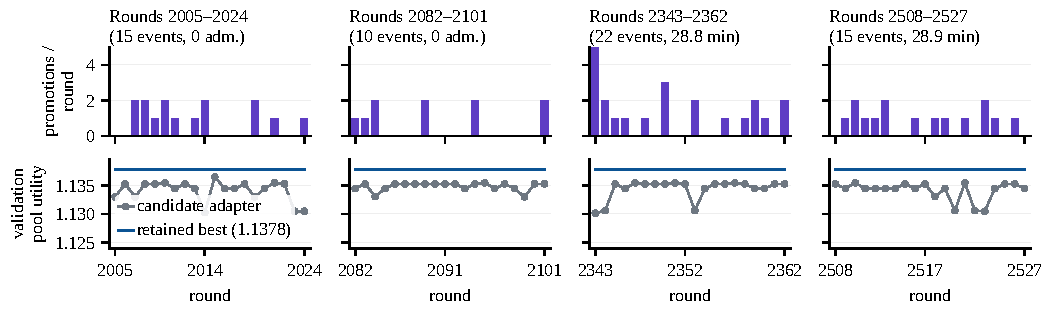
\includegraphics[width=\linewidth,height=2.10in,keepaspectratio]{figures/fig_fw_recent_development.pdf}
  \caption{\textbf{Four 20-round windows record program promotions with zero adapter admissions.}
  Columns show four separate 20-round summary windows: rounds 2005--2024 (15 events),
  2082--2101 (10 events), 2343--2362 (22 events over 28.8\,min of completed-round wall time)
  and 2508--2527 (15 events over 28.9\,min). Top row: strict training-program incumbent
  promotions per completed round. Bottom row: candidate adapter validation pool utility (grey)
  and the post-decision recorded best (blue, \num{1.1378} from round 882). Every window records zero
  adapter admissions. The separate 2644--2663 window is shown once in
  \cref{fig:fw-promotions-per-hour}. Scope: \cref{sec:method-status}.}
  \label{fig:fw-completed-time}
  \label{fig:fw-recent-development}
  \label{fig:fw-followup-development}
  \label{fig:fw-later-development}
  \label{fig:fw-subsequent-window}
  \label{fig:fw-subsequent-utility}
  \label{fig:fw-subsequent-rates}
\end{figure*}
